\section{Cooperative Scheduling Implementation Schemes}
\label{scheme}
%-sequence diagram of what happens in an actor during synchronous and asynchronous method calls.

%\subsection{}
In this section we present how the Java language is used as a backend for ABS and investigate the evolution of the scheme used to implement cooperative scheduling in the Java Runtime environment.  from a very simple approach to using several libraries and features that the latest version of Java provides. The first feature we will use is the Executor interface~\cite{execserv} that facilitates parallel programming in Java. The objects that implement this interface provide a queue of tasks and an efficient way of running those tasks on multiple threads. Throughout this section we will use the terms executor and thread pool interchangeably to refer to this feature. The second notion discussed in our solution was introduced starting with Java 8 and it is the construct for a lambda expression~\cite{lambdas}. This allows us to model a method call as a Runnable or Callable and we will refer to this model as a \textbf{task}. We will look at each solution in terms of four Actor features:

\begin{itemize}
	\item Creation of the actor itself;
	\item Generation of asynchronous calls and message passing;
	\item Releasing control or suspension of a call when encountering an await;
	\item Saving the call stack of a synchronous call upon releasing control.
\end{itemize}



%Conceptually an actor has one thread of execution, which means it can run only one method at a time. Practically, however, allocating a real thread for each actor is highly expensive, as we can have a very large number of actors in the modeled application. Very roughly speaking, an executor service in Java provides a queue of tasks and an efficient way of running those tasks on a few threads. Due to the optimizations provided by Java implementations, an executor in principle is the best way to scale to many concurrent tasks. We use the terms executor and thread pool interchangeably, referring to the main interface~\cite{execserv} that facilitate parallel programming in Java. 

%\subsection{Modeling Language Concepts in the JVM}

\subsection{Every asynchronous call is a thread and each actor has a lock.}
The trivial straightforward approach for implementing cooperative scheduling in Java is for an asynchronous call to generate a new native thread with its own stack and context. We would then model each actor as an object with a lock for which threads compete. The disadvantage here is that this lock-per-actor must be checked by every message handler upon start, and freed upon completion. Whenever an await statement occurs the thread would be suspended by the JVM's normal behavior. When the release condition is enabled, a suspended thread would become available and in turn compete with the other threads in order to execute on the actor. The main drawback of this approach is the large number of threads that are created, which restricts any application from having more method calls than the number of live native threads. Figure~\ref{tp} provides an illustration of this base \textit{process-oriented} approach. Here the idea is that the threads in the circle belong to one actor, thus sharing a lock(the green thread holds the lock, while the red ones are waiting to acquire it). The four Actor features are implemented as follows:

\begin{itemize}
	\item The actor is initialized as an object with a lock;
	\item Asynchronous calls are created as new threads that compete for the lock
	\item Suspension of a call simply suspends the thread;
	\item The call stack of a synchronous call is saved in the suspended thread
\end{itemize}


\begin{figure}
	\centering
	\begin{minipage}{.47\textwidth}
		\centering
		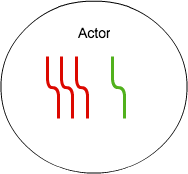
\includegraphics[scale=0.74]{mt.png}
		\caption{Basic process-oriented approach}
		\label{tp}
	\end{minipage}
	\begin{minipage}{.52\textwidth}
		\centering
		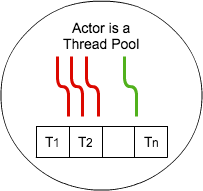
\includegraphics[scale=0.75]{atp.png}
		\caption{Actor-as-executor approach}
		\label{atp}	
	\end{minipage}
\end{figure}

\subsection{Every actor is a thread pool.}
To reduce the number of live threads in an application, we can model each invocation as a task using lambda expressions and organize each actor as a thread pool. This gives the actor an implicit queue to which tasks are submitted. We obtain a small reduction in the number of threads corresponding to the number of tasks that have been submitted, but not started. Once they are started the threads still have to compete for the actor's lock in order to execute, but the number of live threads can be restricted to the number of threads allowed by each Thread Pool, while the rest of the invocations remain in the thread pool queue as tasks. This approach is illustrated in Figure~\ref{atp}. The implementation of the four Actor features is as follows:

\begin{itemize}
	\item The actor is initialized as an object with a lock and a thread pool;
	\item Asynchronous calls are created as new threads that compete for the lock;
	\item Suspension of a call simply suspends the thread;
	\item The call stack of a synchronous call is saved in the suspended thread;
\end{itemize}




%\begin{figure}
%	\centering
%	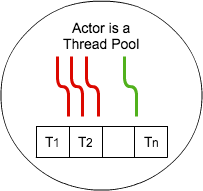
\includegraphics[scale=0.5]{atp.png}
%	\caption{Actor-as-executor approach}
%	\label{atp}	
%\end{figure}

\subsection{Every system has a thread pool.}
In the previous two approaches we modeled the concept of an actor being restricted to one task at a time by introducing a lock on which threads compete. However as all invocations are modeled as tasks that don't need a thread before they start, there is no point in starting more than one task only to have it stuck on the actor's lock. Therefore we introduce \textit{one thread pool per system} or \textit{the system's executor}, and instead of submitting the messages directly to the thread pool, we add an indirection by storing them into an explicit queue first and introduce as a second phase the submission to the thread pool. We assign a separate task for each actor to iterate through its associated queue and submit the next available message to the system thread pool. We will refer to this task from now on as the \textbf{Main Task} of an actor. This removes the requirement to store every message handler as a thread, after it starts and attempts to acquire a lock, saving a task as data in the heap instead.  However it comes at the cost of having to manage message queues manually as we need an explicit queue for all the messages that have not yet been submitted (to the thread pool). 
\par When cooperative scheduling occurs, the executing task of an actor will be suspended and therefore still live in the system as a thread so the application's live threads will be equal to the number of "await" statements in the program. The system's executor can dynamically adjust the number of available threads to run subsequent available tasks, but the application will then still be limited by the maximum number of suspended threads that can exist in the main memory. Furthermore, we still require a lock to ensure that, upon release, the suspended thread will compete with the Main Task associated to the actor from which it originated. This design is presented in Figure~\ref{stp} and it is important to observe the migration of messages into memory and that the red threads are only tasks that have been suspended by an "await". We observe the following changes in the four actor features:

\begin{itemize}
	\item The actor is initialized as an object with a lock, an explicit queue and an implementation of the \textbf{Main Task};
	\item Asynchronous calls are created as new tasks that will be run by the \textbf{Main Task} and will compete for the lock only with suspended tasks;
	\item Suspension of a call restarts the \textbf{Main Task} to iterate the actor's queue and parks the current task as a thread;
	\item The call stack of a synchronous call is still saved in the suspended thread.
\end{itemize}



%We solve the problem by using an indirection, instead of submitting the messages to the thread pool, we add an indirection by storing them into an explicit queue first and introduce as a second pahse the submission to the thread pool.


\begin{figure}
	\centering
	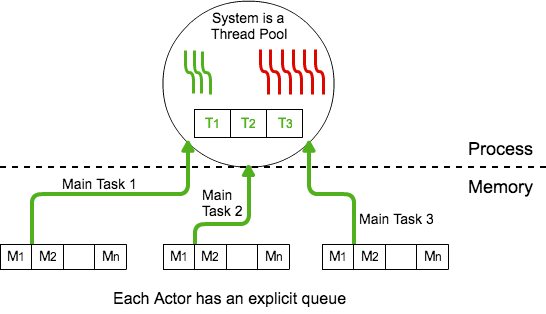
\includegraphics[scale=0.51]{stp.png}
	\caption{System as a thread pool}
	\label{stp}
	
\end{figure}

\subsection{Fully asynchronous environment.}
In the absence of synchronous calls, to eliminate the problem of having live threads when cooperative scheduling occurs, we can also use lambda expressions to turn the continuation of an await statement (which is determined by its lexical scope) into an internal method call and pass its current state as parameters to this method. Essentially what we do is allocate memory for the continuation on the heap, instead of holding a stack and context for it. We will benchmark this trade-off between the memory footprint of a native thread and the customized encoding of a thread state in memory. As there are no more suspended threads in the system to compete with the actor's Main Task, we can eliminate the lock per actor. Finally, let's consider the example in Listing~\ref{ex}. In this case the continuation consists of both the lexical scope of the release statement that is followed by the a complete synchronous call chain that has been generated(i.e. $C(m_2);C(m_1)$). The four features of the Actor are as follows:

\begin{itemize}
	\item The actor is initialized as an object with an explicit queue and an implementation of the of the \textbf{Main Task}, but without a lock;
	\item Asynchronous calls are created as new tasks that will be run by the \textbf{Main Task} and will compete for the lock only with suspended tasks;
	\item Suspension of a call first saves the continuation as a lambda expression guarded by the release condition, and the \textbf{Main Task} continues to iterate through the queue;
	\item The process of saving the call stack of a synchronous call is detailed in the next paragraph.
\end{itemize}



%In this particular scenario the simplest approach is still to save the call stack as a thread and encounter (although to a smaller extent) the same problem as in the previous paragraph. At most, we can give an increased priority to the suspended threads that save call stacks to execute on actors once they are released.
 
%If we assume a fully asynchronous environment then the continuation can always be determined by the lexical scope that follows the release statement. 
 %a separate queue of tasks that are "awaiting" either on a condition or on a future and insert it in

\paragraph{Synchronous calls context.}

In the presence of synchronous calls, the only problem that remains is how to save this call stack without degrading performance? To do this we can try to alter the bytecode to resume execution at runtime from a particular point, but we want our approach to be independent of the runtime and be extensible to other programming languages. Therefore we try to approach the problem differently; if we can turn a continuation, that does not originate from a stack of calls, into a task, is it possible to extend this to synchronous calls as well? We know that this issue arises when methods that contain an "await" statement are called synchronously, but at compile time we can easily identify all of these occurrences from the ABS code. We can simply mark them at compile time and transform them into asynchronous calls followed by an "await" statement on the future generated from the call. Now we can use the same approach for translating these continuations into tasks using lambda expressions and thus eliminating any suspended threads in the system. The final model of our solution is presented in Figure~\ref{sol}. The details of how to construct these continuations and schedule them are presented in Section~\ref{comp}. 
\par A fully asynchronous environment means to change a synchronous call \\ \lstinline|x = this.m();| into an asynchronous call plus an await like \lstinline|f = this!m();| \\ \lstinline| x = await f?;|. There are two problems here. First, we still need to make sure that "m" must be the exact next method that will run. Second, when "m" finishes, the actor scheduler must immediately schedule the method that is waiting for its result. Both can be implemented by changing the non-deterministic behavior of the Main Task. There are two constrains that we have to impose to preserve the chain of synchronous calls. First, we set a flag "isSyncCall" in the task that is calling "m" and when that flag is true, the Main Task will immediately execute the message that is to be enqueued instead of taking an arbitrary one from the queue. Second, assuming that there is no "message overtaking", the messages that are part of a synchronous call chain arrive in the Actor's queue in the FIFO order. We can label each call chain with a number "syncContext" and all messages part of that call chain will have this number. When the Main Task completes a message labeled with a particular number it will take from the queue the next available message with the same label and execute it. Finally, when the last message with that label is complete, then the call chain is complete and the next message will be selected arbitrarily.

\begin{figure}
	\centering
	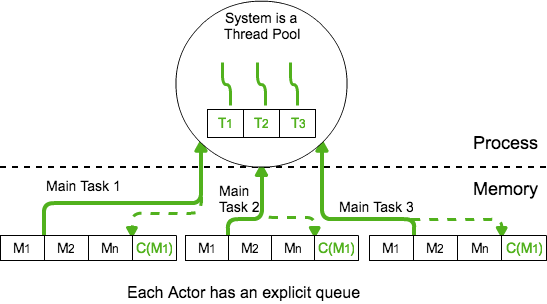
\includegraphics[scale=0.47]{solution.png}
	\caption{Full data-oriented approach}
	\label{sol}
\end{figure}

%\subsection{Optimizations for the JVM}
%\label{optimizations}
%We investigate the performance impact of eliminating the large number of expensive threads in Java that are required to implement the cooperative scheduling model. Using this data-oriented approach for saving contexts we limit any application to the system's main memory size, but added to that we also obtain some other optimizations related to Java's features.
%
%\paragraph{Demand-driven approach.}
%An important advantage of having a task assigned to each actor and a manually processed queue is that we can start and stop the task depending on the queue state. To avoid keeping the Main Task alive, we make it part of the functionality of sending a message or completing a future to notify the Main Task. This is done by any other actor who sends an invocation to an empty queue and subsequently the Main Task stops when there are no more enabled messages in the queue. This gives rise to some subtle synchronization points that will be detailed in Section~\ref{run}. An important observation to make here is the two scenarios that re-enable tasks. These release points may occur when actors fulfill a future and therefore we require the system to have a notification mechanism for actors with empty queues and newly enabled messages which we will detail in Section~\ref{run}. This requires maintaining a global hash table, mapping every future to the set of actors that are awaiting on its completion. When release points occur due to an internal state becoming valid, the Main Task is responsible for verifying the boolean condition before it may end (possibly because of no enabled messages), so no special notification is required in this case.
%
%%As ABS semantics do not allow actors to modify each other's internal state, we know that a release point that will validate a boolean condition based on a change of an actor's state can only occur during another task that is already executing on that actor. This release point will always occur before the running task ends and therefore the queue can never be empty as the released message will be available in the queue and no special notification will be required to resume the task assigned to the actor. 
%
%
%\paragraph{Optimal usage of system threads.}
%The approach of using one thread pool per system gives the user direct control over the number of live threads the application creates. Using the Executor interface in Java allows the user to choose the type of thread pool that manages the actors and set the maximum number of threads that are available. For example the user can limit the number of threads the application has to the number of cores that the machine provides and avoid context switches made by the JVM. This in turn means that the implementation has to provide fair usage of the threads with respect to the Main Tasks that run the actors, an issue which we will also touch upon in Section~\ref{run}. 
%
%\paragraph{Eliminating busy waiting.}
%Cooperative scheduling through the "await" statements may suspend the current message run by the actor based on either a particular inner state or future requiring completion on a different actor. We discussed how the Main Task can start or stop based on release points, but how exactly does an actor verify that a release point has completed? Clearly, having a task continuously iterate through all suspended messages (busy-waiting) is inefficient. While we can permanently mark a message that needs a future to complete as available, by the nature of ABS, we cannot do that for a message which is released by a particular valid state, as its state can change again by the time it is run, so it always has to be verified before it is fetched. Instead, we assign this verification to the Main Task that iterates through the queue, and simply stop the task if no message is available. If the task does stop, it means that the actor is in a state in which it is unable to execute any of its suspended messages. Therefore, it requires another actor to either send a new invocation that will change its state or the system to send a notification about a future that may release some of its messages and re-enable the Main Task. 
%
%
%\paragraph{Using JVM Garbage Collection}
%Using the approach explained so far in this section, the only extra references we need for the actors are the ones inside the global hash-table required for the notification mechanism for futures. Once the future is completed and notifications are sent, the key is deleted and the actor references become unreachable. Therefore we can leave the entire garbage collection process to the Java Runtime Environment as no other bookkeeping mechanisms are required.

